% Preamble
% ---
\documentclass{article}

% Packages
% ---
\usepackage{amsmath} % Advanced math typesetting
\usepackage[utf8]{inputenc} % Unicode support (Umlauts etc.)
\usepackage{hyperref} % Add a link to your document
\hypersetup{
    colorlinks=true,
    linkcolor=black,
    filecolor=black,
    citecolor=blue,
    urlcolor=blue,
}
\usepackage{graphicx}
\usepackage{caption}
\usepackage{draftwatermark}
\SetWatermarkText{DRAFT}
\SetWatermarkScale{.8}
\usepackage{fancyhdr}
\pagestyle{fancy}
\fancyhf{}
\fancyfoot[L]{\small\textit{Draft – Confidential – Do Not Distribute}}
\renewcommand{\headrulewidth}{0pt}
\usepackage{listings}
\usepackage{lmodern}
\usepackage{framed}
\usepackage{appendix}
\usepackage{csquotes}
\usepackage[letterpaper, portrait, margin=1in]{geometry}
\usepackage{multicol}
\usepackage{parskip}
\usepackage{ragged2e}
\usepackage{tabularx}
\usepackage{indentfirst}
\graphicspath{ {../images/} }


\begin{document}

\begin{titlepage}
  \begin{center}
    \vspace*{0.15\textheight} % Adjust vertical centering (top padding)

    {\LARGE \textbf{XYO Layer One Blockchain White Paper}}\\[1.5cm]

    {\large Arie Trouw, Joel Carter, Matt Jones, Jordan Trouw\footnote{XYO – arie.trouw@xyo.network, joel.carter@xyo.network, matt.jones@xyo.network, jordan.trouw@xyo.network}}\\[0.8cm]

    {\normalsize June 2025}\\[2cm]


    \begin{center}
    \line(1,0){50}
    \end{center}

      \begin{abstract}
        \noindent
        XYO Layer One (XYOL1) is the first blockchain designed specially for high-throughput data, which allows for a truly scalable ecosystem while maintaining speed and efficiency. Using the XYO Layer One Protocol, the blockchain addresses multiple existing limitations in the current blockchain landscape, namely issues with data sovereignty and cryptographic bloat, through technological features such as Lookback Windows, Step Hashes, Rollups, Framing Cursors, Bound Witness Trees, Bearer Proofs, and Proof of Perfect.\footnote{These features are explained in depth in Section 3.} Through XYO Layer One Blockchain, separate XYO Proof of Origin Chains\footnote{See XYO White Paper, pub. 2018.} can be bound into a decentralized, consensus driven, shared state. This shared chain is built and managed by a network of staked nodes that follow this protocol.
      \end{abstract}

    \vfill % Push everything above toward vertical center, while keeping footnotes at bottom
  \end{center}
\end{titlepage}


%Introduction
\section{Addressing Known Issues in Blockchain}
XYO Layer One, both a blockchain and a protocol, addresses one of the biggest issues in today's blockchain landscape: the ever-increasing size of the chain itself. Nearly all existing layer one blockchains are predicated on a single shared state between every node running the chain. This shared state includes everything from the genesis block to the latest block created.\footnote{The “genesis block” is the very first block in a blockchain, serving as the foundation for all subsequent data.} In this structure, every requested blockchain value requires the history of the entire chain, which gets increasingly larger as the blockchain is built. This is the issue of blockchain bloat.

\subsection{The Consequences of Blockchain Bloat}
Multiple structural and integrity issues arise as a result of increasing block sizes, including increased requirements for blockchain compute, slower block speeds, difficulty with historical data integrity, increased environmental toll, and network latency. Every new block takes more energy, is slower to build, and impacts the efficiency of the chain. The rising computational demands for engaging with blockchain technology also make participation inaccessible to everyday individuals and independent developers. Instead, participation concentrates among large corporations and nation-states that can afford to use off-chain fiat resources to seize control of blockchain ecosystems—undermining the core principles of decentralization and equal access. 

\subsection{The XYO Layer One Solution}
XYO Layer One Blockchain does not require every block to maintain a full state of the entire chain. As a single, consensus-driven Proof of Origin chain, it offers a novel solution to blockchain bloat, effectively and efficiently addressing the previously listed issues. This solution is achieved primarily through the use of Lookback Windows and Step Hashes, and is further enhanced through ZKRollups, Framing Cursors, Merkles, and Bearer Proofs.\footnote{These technical features of XYO Layer One are discussed in Section 3.}

With these improvements, XYO Layer One's active set of data required to create and validate new blocks is reduced substantially and does not grow over time after a certain size is reached. This solves the storage problem that makes most layer one block chains unusable for many data-reliant applications, such as DePIN (Decentralized Physical Infrastructure Networks), Artificial Intelligence, Real World Assets (RWA), Machine Learning, Telecommunications, Healthcare, Finance, Logistics, and more. 

\begin{center}
    \line(1,0){50}
\end{center}

\section{Elevating the Original XYO Protocol}
The original XYO Proof of Origin Protocol defined in the 2018 White Paper provided immutability, traceability, and data validation for singular data sources. This offered a universal and fully-sovereign solution for many industries, but also resulted in isolated XYO Proof of Origin chains that lacked a shared state. These individual chains occasionally co-signed a shared Bound Witness\footnote{See Section 2.1 for details on Bound Witnesses inside XYO Layer One.}, effectively “entangling” the chains, but there was no representation of the collective state across multiple XYO Proof of Origin Chains as a whole. 

The new XYO Layer One Protocol defines a method for a ”Chain of Chains” allowing for a single collective state built from individual XYO Proof of Origin Chains. The new Protocol opens the door for a public XYO Layer One Blockchain that ensures verifiable, collectively-immutable state from individually sovereign data sources. 

With the XYO Layer One Protocol, the following features become available for the XYO Layer One Blockchain: 

\begin{enumerate}
    \item XYO Token Staking for participation rewards 
    \item A native token for gas and payments of services and data in real time
    \item A consensus-driven shared reality that unifies the isolated Proof of Origin chains that exist in XYO today
\end{enumerate}

\subsection{Bound Witnesses as Core Components of XYO Layer One}
Bound Witnesses were originally defined in the 2018 XYO White Paper. Unique to XYO, Bound Witnesses are a core part of the XYO Layer One infrastructure and enable many of the features and benefits of the XYO Layer One Blockchain. 

\subsubsection{Defining Bound Witnesses}
In short, Bound Witnesses represent “bundles” of data that are signed by 1 or more XYO Nodes to prove validation from 1 or more data parties. Bound Witnesses can contain a variety of data and normally follow designated “Schemas” that define the structure and requirements of a specific type of Bound Witness. 

XYO Layer One still uses many familiar blockchain elements like blocks and transactions, but structures them as Bound Witnesses. For instance, instead of using a traditional block format, each block is a special kind of Bound Witness with fields specific to blocks in XYO Layer One. These Block Bound Witnesses link back to previous blocks using cryptographic hashes, allowing anyone to walk through the chain and verify the origin of data. This linking mechanism and multi-party signature architecture are what tie XYO Layer One directly to its original Proof of Origin protocol.

\subsubsection{Payload Elevation to a Bound Witness}
XYO Layer One introduces a new concept for Bound Witness and Payload interaction: Elevation. Payload Elevation is the act of “elevating” a payload to be included in a Bound Witness, thereby adding permanency to both the hash and the data it relates to. This permanency is done via the Bound Witness's Proof of Origin Chain.

In the XYO Layer One Blockchain, these elevations are most commonly found between Transaction Bound Witnesses and Block Bound Witnesses.\footnote{Transaction and Block Bound Witnesses are described in detail in Section 8, “Block Structure”.} In these cases, Transactions use scripts, similar to Ethereum's Smart Contracts, to designate Payloads for elevation. When they're elevated, they're packaged into the current Block, which is also a Bound Witness, and then stored as part of the chain.

\begin{center}
    \line(1,0){50}
\end{center}

\section{Consensus Protocol and Unique Rewards}
XYO Layer One uses a variant of Proof-of-Stake (PoS) as its consensus mechanism, with an added emphasis on \textbf{Proof of Participation}\footnote{See Section 8 for details on Participation Transactions and Validator Eligibility.} to fairly reward active contributors. Stake size serves as the foundation of trust in the network: it governs which actors are eligible to produce or validate blocks and how much influence they can exert. Trust in XYO Layer One is currently based on stake size and active participation, not on the historical age of the node or its prior activity. This helps simplify the trust model and avoid legacy advantages or bias toward older nodes.

Unlike traditional PoS systems where Validator Node staking alone often suffices, XYO Layer One \textit{requires Validators to submit on-chain participation transactions} in order to qualify for rewards in the Step Reward Pool.\footnote{See Section 12 for Step Reward Pool details.} This ensures that only actively engaged nodes are compensated, helping maintain both performance and accountability across the network.

In addition to Validators and Block Producers, \textbf{System Stakers}\footnote{See Section 11 for System Staking} (users who delegate their stake without running a node) can also earn rewards from the Step Reward Pool at a lower rate. This structure supports a broad range of contributors while preserving strong incentives for Validators and Block Producers, who perform protocol-level duties and assume slashing\footnote{See Section 11 for Slashing Conditions and Participation Requirements.} risk for misconduct or inactivity. Detailed reward models, including the 2-part reward system with the Step Reward Pool alognside Block Rewards, and slashing conditions are described in later sections


\begin{center}
    \line(1,0){50}
\end{center}

\section{XYO Layer One Blockchain Features}
TXYO Layer One introduces several novel and existing features to address the challenges of blockchain bloat, scalability and performance. These features enable a better blockchain solution suitable for data-intensive industries like AI, RWA, and DePIN. 

\begin{itemize}
    \item \textbf{Lookback Window:} Reduces the amount of historical data that needs to be maintained and analyzed for each block. 
    \item \textbf{Step Hash:} Allows for efficient grouping and retrieval of blocks, improving data access speed and reducing storage requirements. 
    \item \textbf{Rollups:} Bundles multiple transactions into a single proof, reducing the amount of data stored on chain and improving scalability.
    \item \textbf{Bound Witness Trees:} Organizes transactions into a tree structure for efficient verification and scalability. 
    \item \textbf{Framing Cursors:} Optimizes data retrieval by segmenting the blockchain into manageable sections.
    \item \textbf{Bearer Proofs:} Provides cryptographic proof of data inclusion in a set without needing the entire containing set. 
    \item \textbf{Proof of Perfect:} Algorithmic proof that ranks items such as chain heads in order of perfectness.
\end{itemize}

Together, these concepts reinforce one of the biggest paradigms of XYO Layer One: off-chain data, on-chain proof.

\subsection{Lookback Window}
In XYO Layer One, block building, validating and indexing become more efficient through the concept of a “Lookback Window”. A Lookback Window refers to the amount of previous blocks across which block builders and validators need to maintain to operate within the network. 

\subsubsection{Current Blockchains}
Most blockchains have a Lookback Window equal to the length of the entire chain — in order to analyze the chain for data, a node must scan the full length of the chain. Although this allows for consistent access of all historical data, it comes at the expense of larger compute and storage requirements.

\begin{center}
    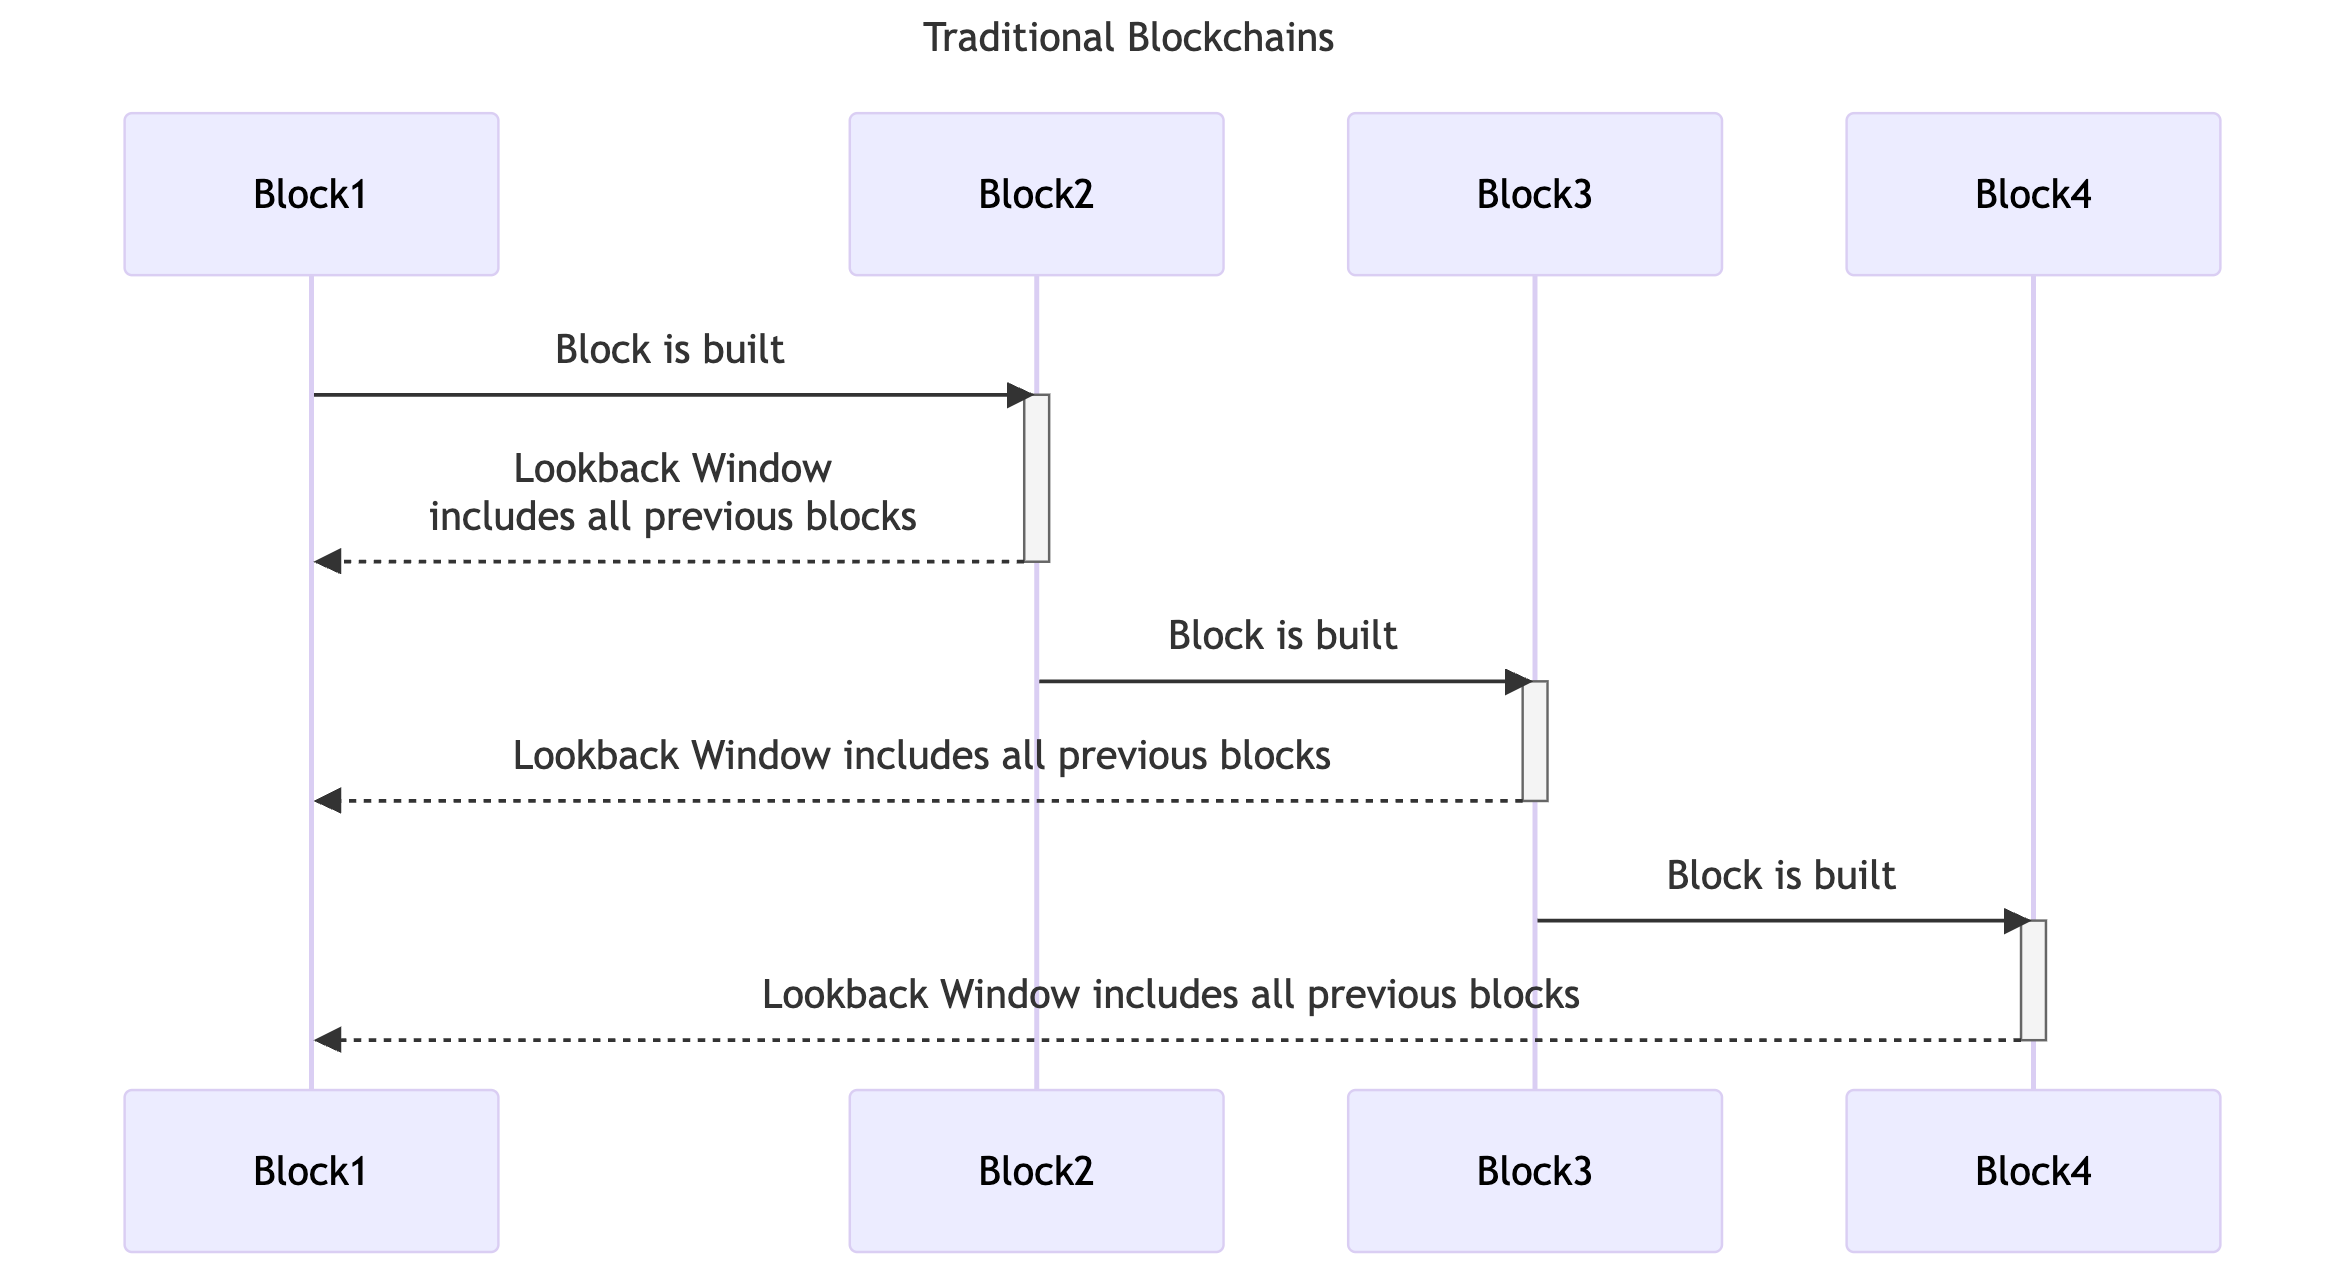
\includegraphics[width=15cm]{trad-blockchain-lookback-window.png}
\end{center}

With the precondition that each node maintains and analyzes a complete record of the entire blockchain, the requirements for network participation grow in an ever increasing fashion. This has led to an erosion of the decentralization for blockchains that have been operational long enough to realize this effect, as network participation by enthusiasts has been superseded by the few participants who can afford high-end hardware, and network indexing has been outsourced to centralized Web2 services.

\subsubsection{The Lookback Window Solution}
XYO Layer One contains an advanced Lookback Window algorithm that allows for variable Lookback Windows. This feature optimizes blockchain operations by focusing on the most recent N transactions—such as the last 10,000 or 1 million—actively used to maintain the system. Each node is only required to store these recent transactions, significantly reducing storage requirements and boosting transaction speeds. Older transactions are stored in a backup system, ensuring minimal disruption to performance while still allowing easy access when needed. 

\begin{center}
    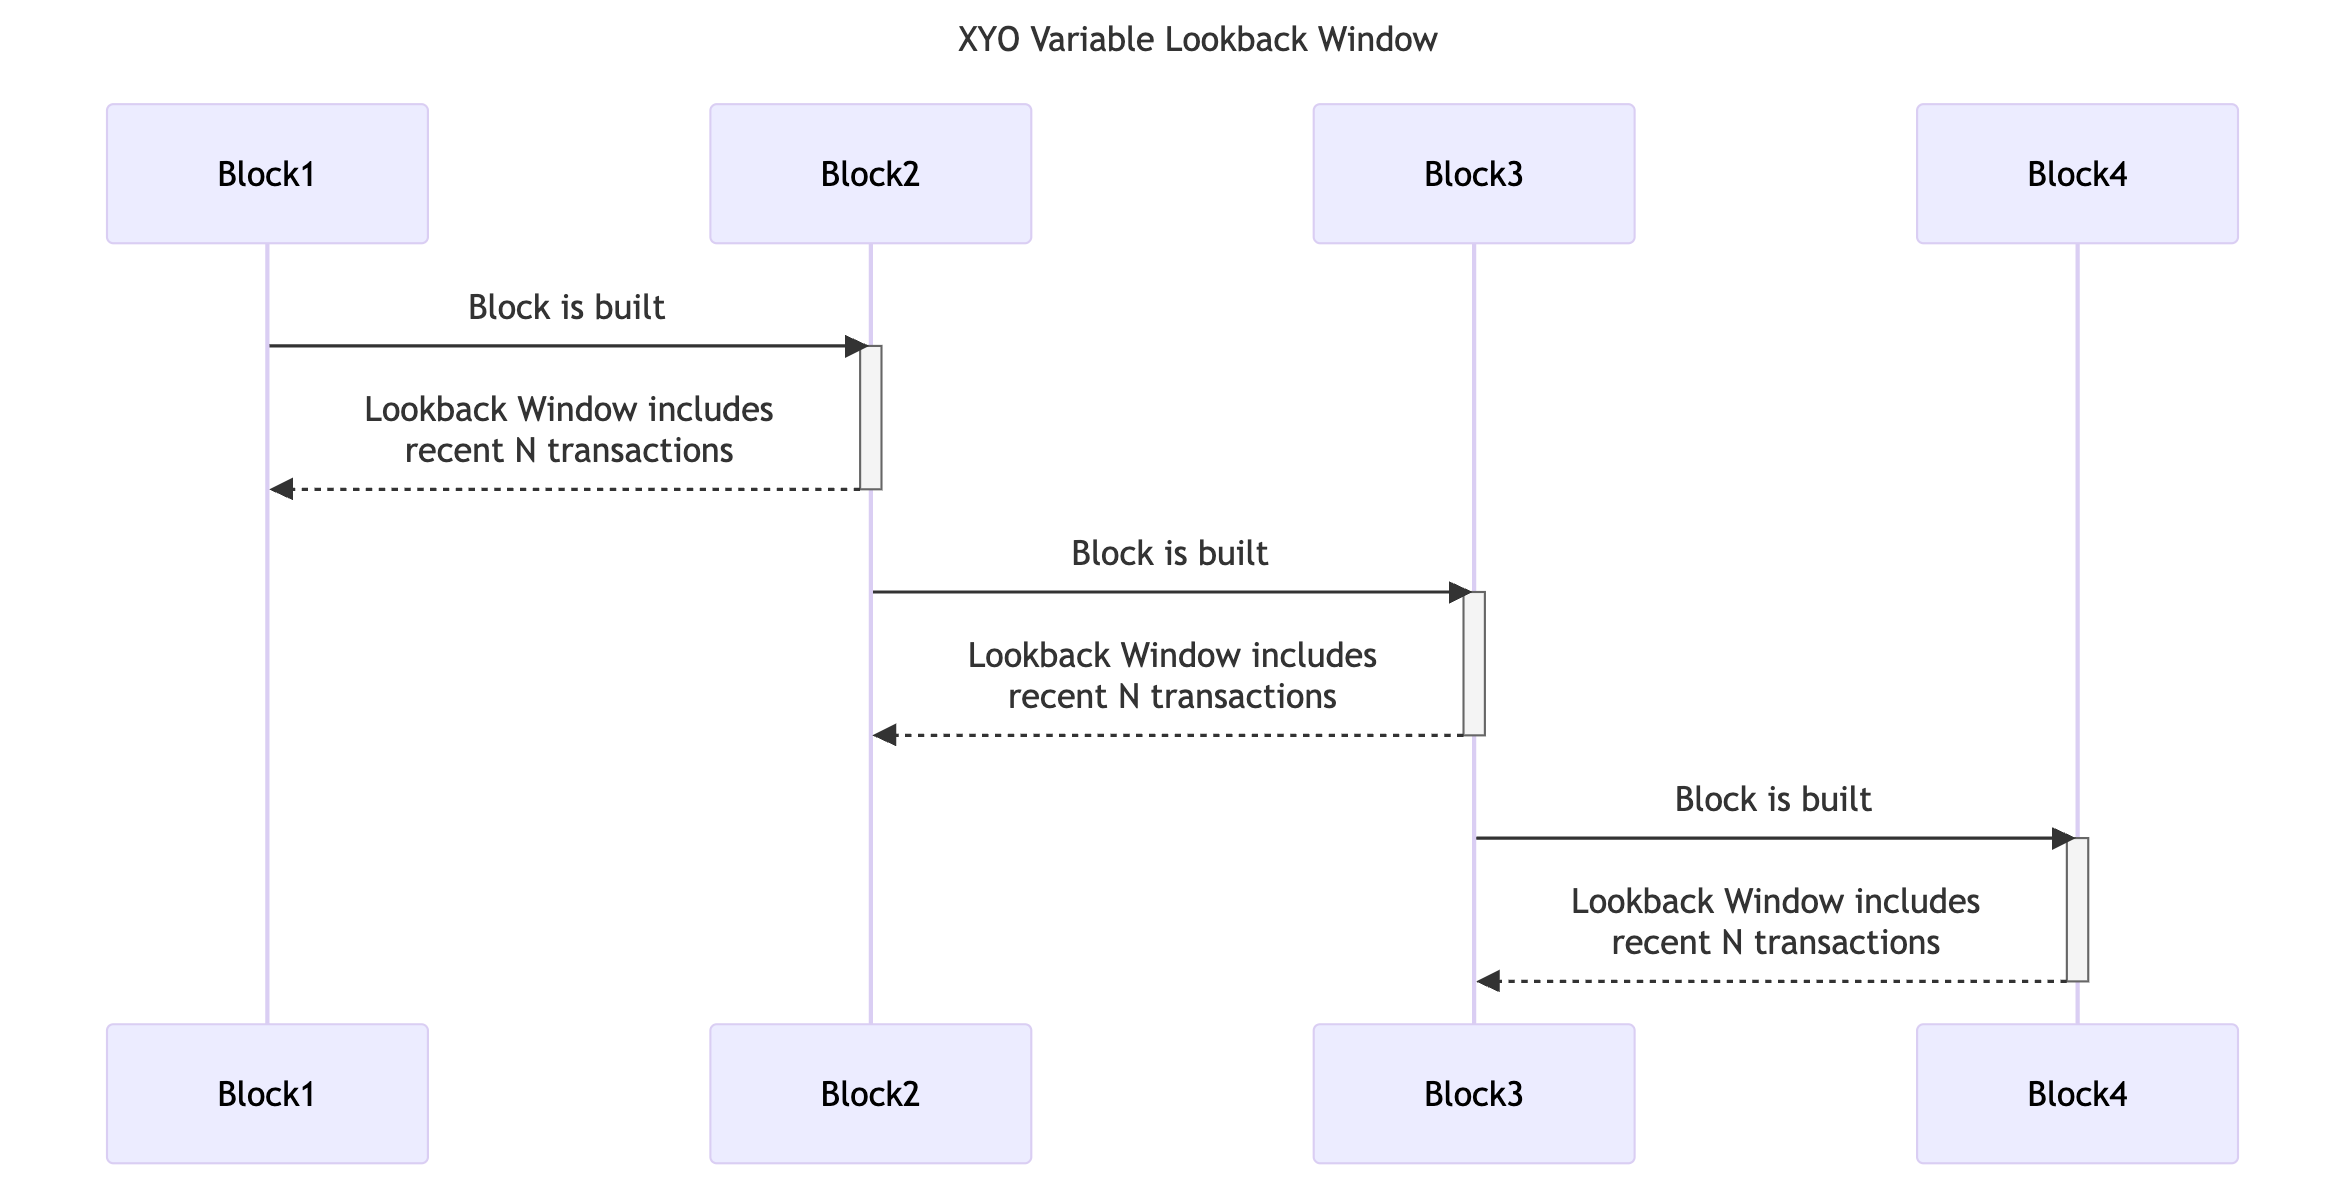
\includegraphics[width=15cm]{xyo-variable-lookback-window.png}
\end{center}

This approach contrasts with traditional blockchains like Bitcoin and Ethereum, where nodes must store the entire blockchain history as well as maintain and index historical global state such as UTXOs\footnote{Unspent Transaction Outputs (UTXOs) are cryptocurrencies in an address that have not yet been spent.} or Address Balance, leading to ever increasing hardware requirements and inefficiencies as the network grows. XYO's Lookback Window ensures scalability and speed, allowing for faster processing and more efficient use of resources as the blockchain scales, setting the foundation for a more robust and responsive decentralized ecosystem. 


\subsection{Step Hash}
Step Hashes in the XYO Layer One Blockchain significantly improve the efficiency of locating data contained within the blockchain. Unlike traditional blockchains, which can sometimes require a full walk of the entire chain to verify included data, Step Hashes group blocks together into multiple segments of progressively larger sizes. The varying group sizes allow for faster searches, as you can first check the group hashes and then zoom into specific blocks within that group. Instead of checking blocks one-by-one, Step Hashes enable giant steps through the blockchain, making it easier and more efficient to access the oldest parts of the chain. This innovation enhances both speed and scalability, setting XYO Layer One apart from other blockchain systems.

\begin{center}
    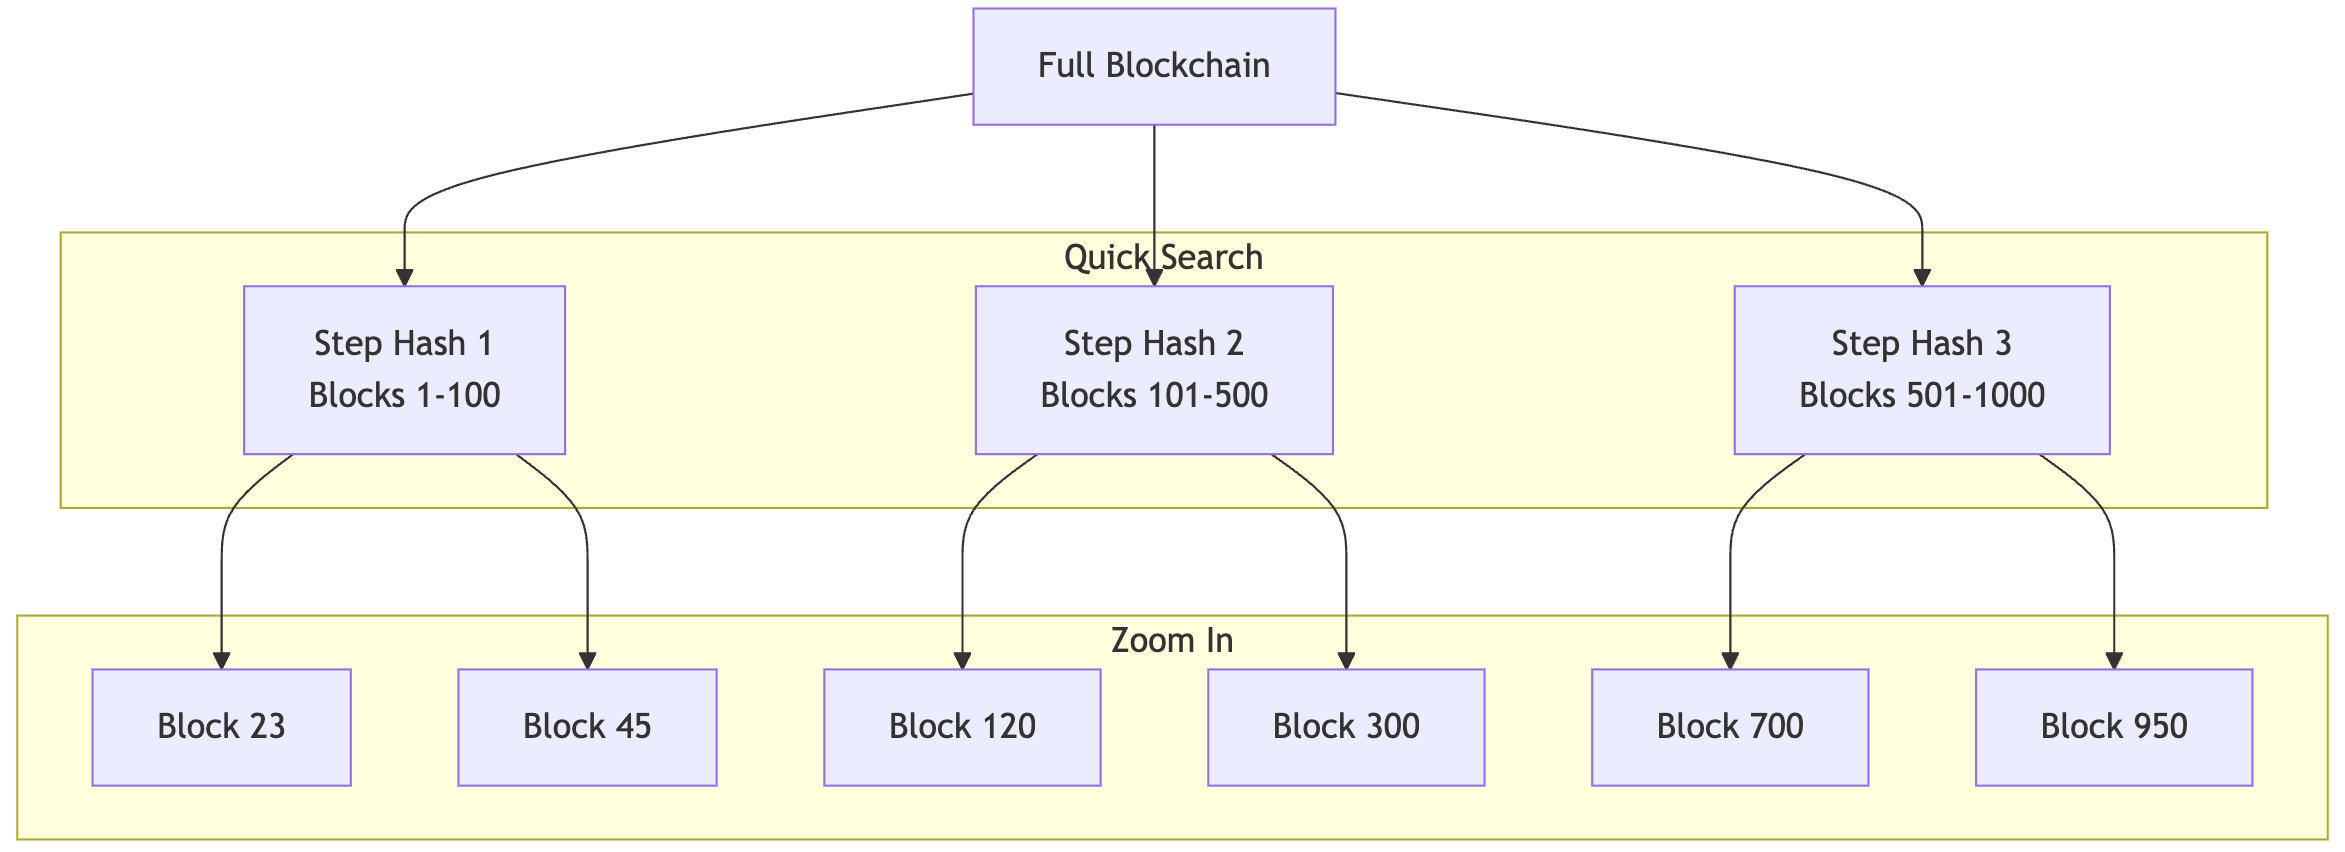
\includegraphics[width=15cm]{step-hash.png}
\end{center}

\subsection{Rollups}
Rollups are a crucial feature for enhancing the scalability and performance of the XYO Layer One Blockchain, particularly in industries requiring high volumes of data processing such as AI, Machine Learning, and DePIN. 

Instead of processing every transaction directly on the blockchain, Rollups bundle multiple transactions together off-chain and then submit a summarized proof of these transactions to the main blockchain. This proof ensures that the transactions are valid and optionally without revealing sensitive data. By doing this, Rollups help reduce the amount of data stored on the blockchain. This approach significantly reduces the computational load and storage requirements of the base layer. 

\begin{center}
    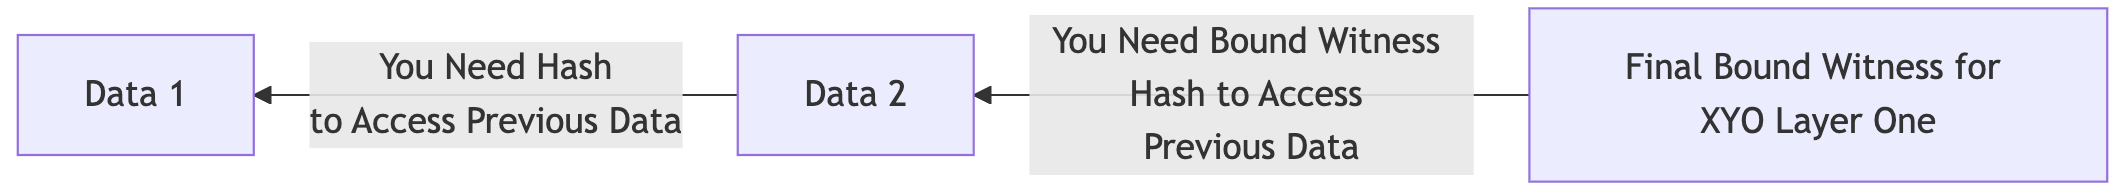
\includegraphics[width=15cm]{rollup.png}
\end{center}

The key features of Rollups in XYO Layer One include: 
\begin{itemize}
    \item \textbf{Off-chain transaction bundling:} Multiple transactions are processed off-chain and bundled into a single batch, reducing the number of individual transactions that need to be processed on-chain.
    \item \textbf{Zero-Knowledge Proofs (ZKPs):} These cryptographic proofs are used to verify the correctness of off-chain transactions without revealing the underlying data, ensuring both privacy and security. 
    \item \textbf{Efficiency and reduced transaction costs:} By submitting only proofs to the blockchain, Rollups minimize on-chain data, improving throughput and lowering transaction costs.
\end{itemize}

\subsection{Bound Witness Trees}
Bound Witness Trees are a type of Rollup that contains one or more Bound Witnesses. They are a foundational component of XYO Layer One, enhancing the data organization and efficiency of the chain. By organizing transactions and data into a tree-like structure, where each leaf node contains a hash of a transaction and non-leaf nodes aggregate these hashes, Bound Witness Trees enable quick and efficient data verification. 

\begin{figure}[ht]
    \centering
    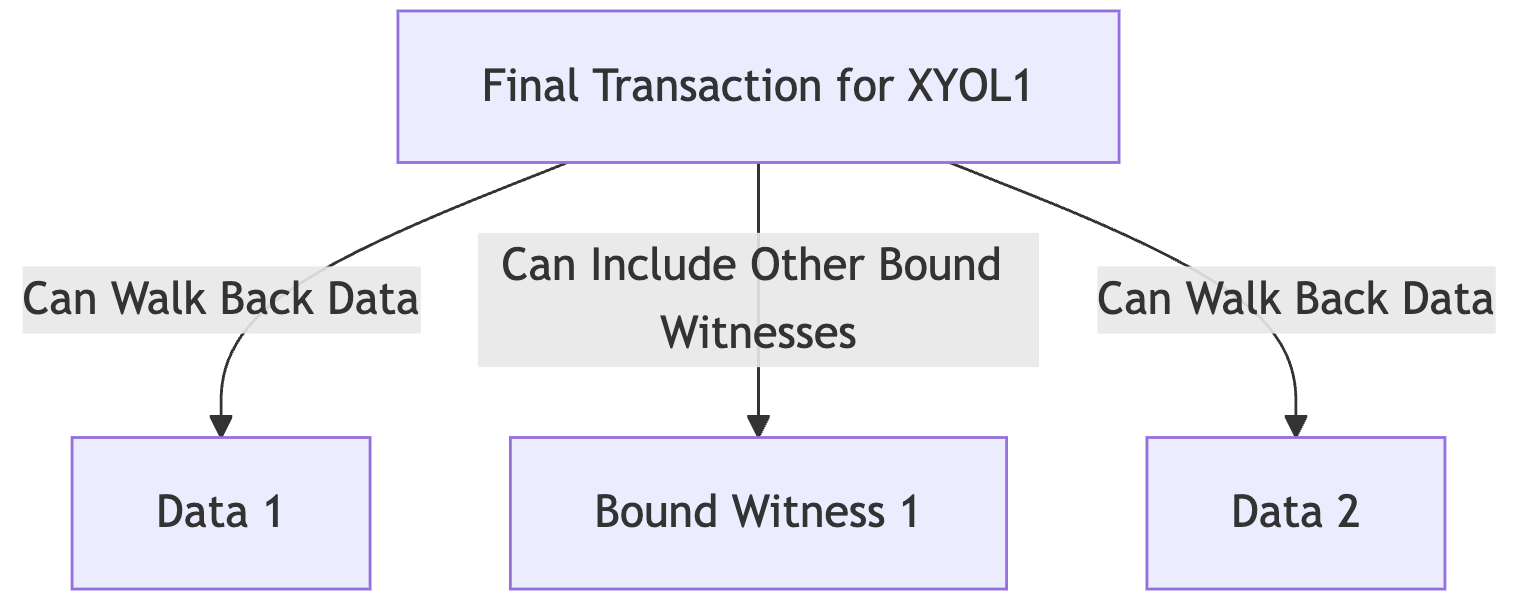
\includegraphics[width=15cm]{bound-witness-trees.png}
    \caption{Bound Witness Trees make data compression for blockchain simple and easy to retrieve}
\end{figure}

In XYO, this structure improves scalability by allowing nodes to verify large datasets with minimal computation. Only the Bound Witness root needs to be stored and compared, reducing the amount of data that must be processed for transaction validation. This enables faster transaction verifications and significantly reduces the storage and computational load on the network, making the XYO Layer One Blockchain both more efficient and scalable.

\subsection{Framing Cursors}
Framing Cursors are a key feature in the XYO Layer One Blockchain that optimize the process of accessing and validating data across large-scale decentralized networks using Step Hashes. They act as pointers or markers that help navigate the blockchain more efficiently by segmenting the blockchain into manageable “frames” or sections. This allows for targeted data retrieval rather than performing a full scan of the entire blockchain. 


\begin{figure}[h]
    \centering
    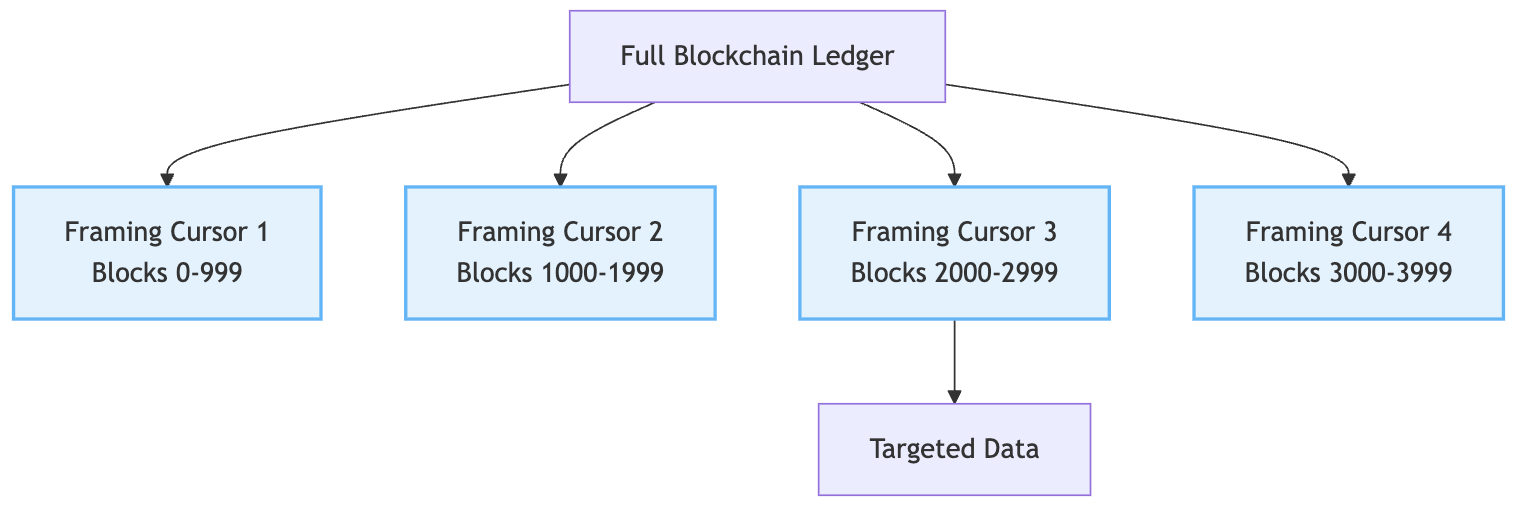
\includegraphics[width=15cm]{framing-cursor.png}
\end{figure}

By using Framing Cursors, XYO reduces the computational load required to find relevant data, enabling faster query responses and improving overall blockchain performance. This mechanism is particularly useful as the network scales, ensuring that data retrieval remains efficient even as the blockchain grows in size. 

\subsection{Bearer Proofs}
\begin{minipage}[t]{0.45\textwidth}
\raggedright
Bearer Proofs play a crucial role in enhancing data integrity and verification within the XYO Layer One Blockchain. This cryptographic proof allows for the verification of ownership and authenticity of data without exposing the data itself. Bearer Proofs are particularly useful in ensuring that the information being transmitted or stored on the blockchain is legitimate and unaltered.

In XYO, Bearer Proofs enable more efficient data validation by providing a secure and lightweight way to confirm data ownership, thus reducing the need for full access to the underlying data. This leads to faster, more secure transactions, contributing to both the scalability and security of the XYO ecosystem.

\end{minipage}%
\hfill
\begin{minipage}[t]{0.42\textwidth}
\centering
\vspace*{-2.5em} % move image up if needed
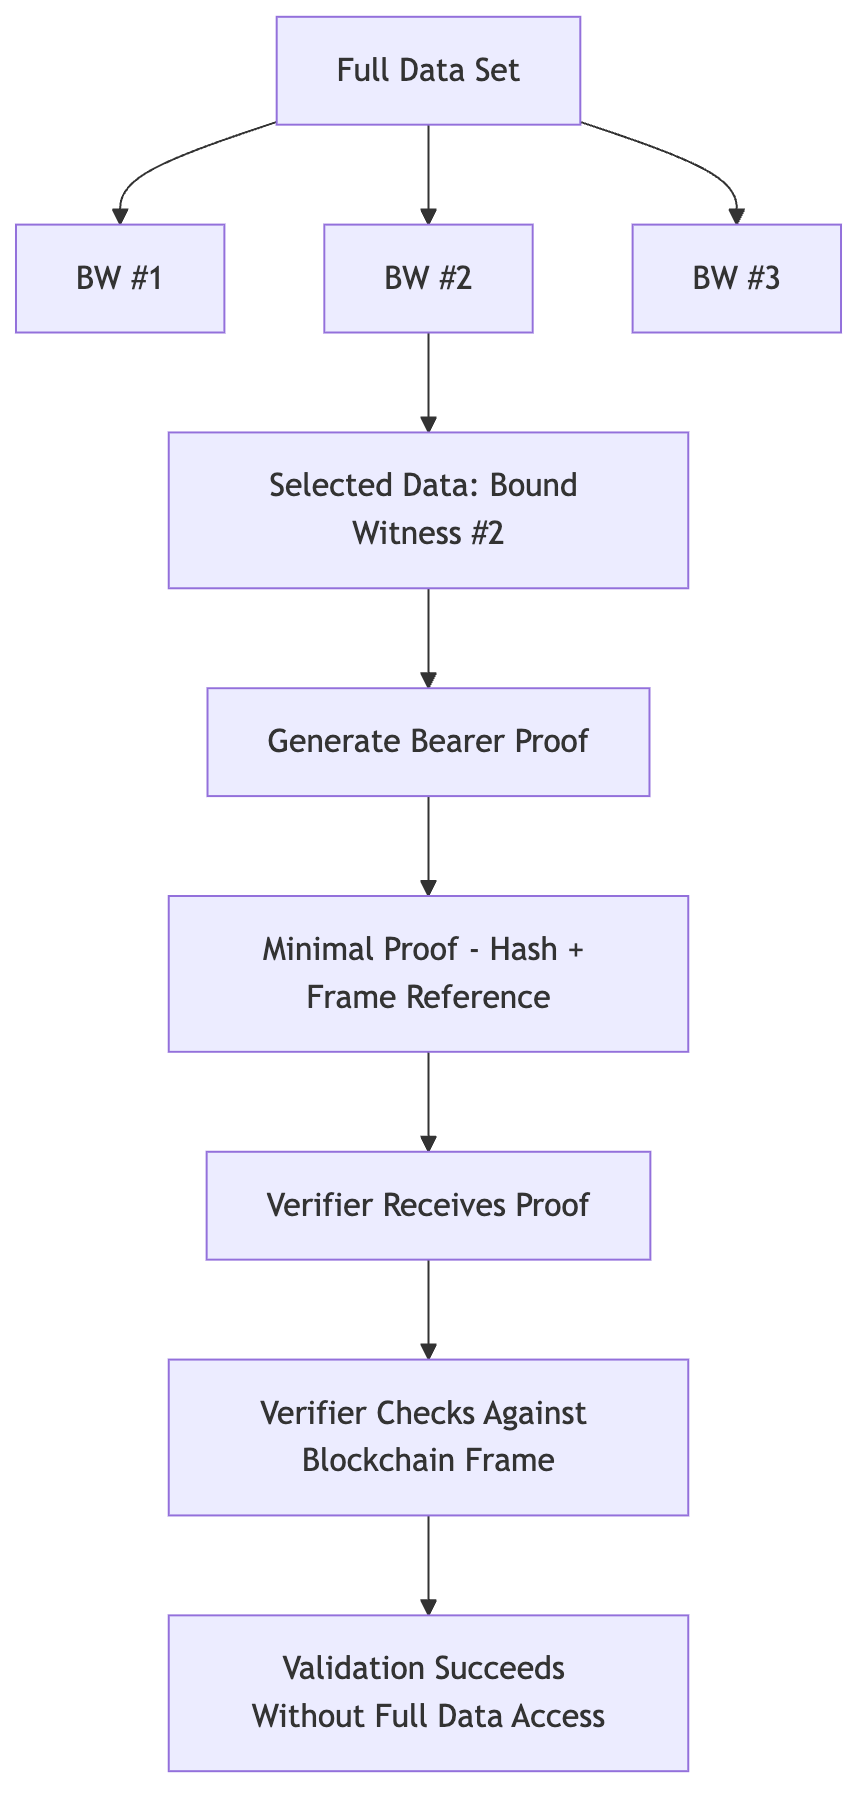
\includegraphics[height=12cm]{bearer-proof.png}
\vspace{0.5em} % space between image and caption
\end{minipage}

\subsection{Proof of Perfect}
Proof of Perfect is a novel data-ranking algorithm used within XYO Layer One to identify and prioritize the most accurate and reliable data available—such as chain heads—based on their relative “perfectness.” In decentralized systems, pinpointing a single “perfect” data point can be inherently difficult, especially when data is collected from multiple, diverse sources. Rather than assuming absolute perfection, Proof of Perfect evaluates each candidate against others, algorithmically ranking them by proximity to an ideal.

This comparative approach enables the network to consistently select the most trustworthy data, even in complex or imperfect environments. As more data points become available, the algorithm's accuracy improves, making it increasingly effective in identifying the best possible option. By promoting better data quality, ensuring accuracy even in uncertain conditions, and scaling with the network, Proof of Perfect reinforces XYO Layer One's ability to utilize trustworthy, high-integrity data at scale.

\begin{figure}[h]
\centering
\begin{minipage}[t]{0.48\textwidth}
    \centering
    \vspace{0pt}
    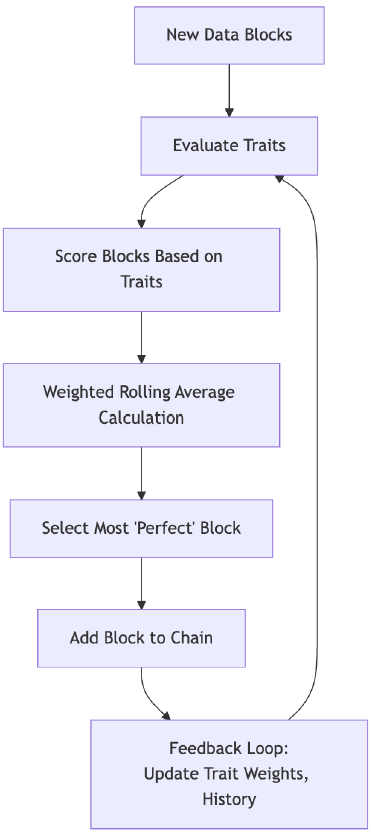
\includegraphics[height=10cm]{proof-of-perfect-flow.png}
    \caption{Proof of Perfect uses a feedback loop to evaluate traits to determine whether or not data is added to the chain.}
\end{minipage}
\hfill
\begin{minipage}[t]{0.48\textwidth}
    \centering
    \vspace{0pt}
    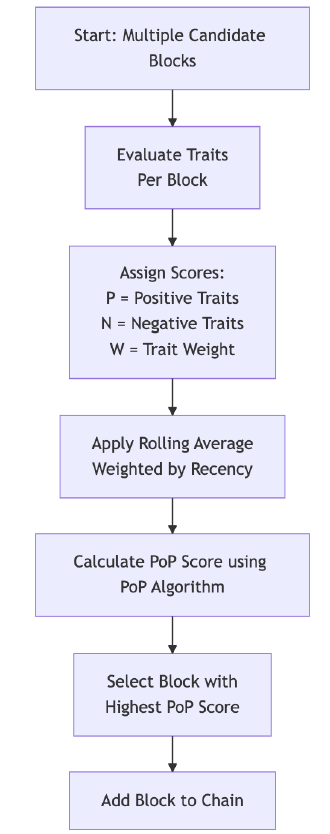
\includegraphics[height=10cm]{proof-of-perfect-algorithm.png}
    \caption{Proof of Perfect is defined by an algorithm using variable positive and negative traits.}
\end{minipage}
\end{figure}

\begin{center}
    \line(1,0){50}
\end{center}

\section{XL1 Token}
The XL1 Token is the native currency of the XYO Layer One Blockchain, primarily used for transaction fees, gas fees, and incentivizing network participants. XL1 plays a crucial role alongside the XYO Token in ensuring the scalability and efficiency of the XYO ecosystem by enabling transactions, rewarding participants, and securing the network through staking. 

\subsection{Purpose}
The XL1 Token serves multiple functions within the XYO Layer One Blockchain: 

\begin{itemize}
    \item \textbf{Transaction Fees}: XL1 is used to pay for transaction processing, covering the computational costs of transactions and services.\footnote{See Section 9.2 for breakdown on Transaction Fees and details on Gas.}
    \item \textbf{Gas Fees}: XL1 powers blockchain operations, particularly by covering the gas required for the execution of smart contracts and validation of transactions.
    \item \textbf{Incentives}: XL1 is used to reward block producers, validators, and other network participants for their contribution to the network.
\end{itemize}

\subsection{Usage}
XL1 is used as a block reward mechanism for incentivization within XYO Layer One Blockchain. It can also be transferred between addresses for:
\begin{itemize}
    \item \textbf{Payments} – Used for services like storage and compute.
    \item \textbf{Gifts} – Sent without contractual obligations.
\end{itemize}

\subsubsection{Lookback Window Rule}
To prevent balance inconsistencies, XL1 transactions must be within the
\textbf{Current Lookback Window} of the producer validating the transaction. If
an address has XL1 outside the window, it must refresh its balance before
transferring.\footnote{See Section 4.1 for details on Lookback Windows.}

\subsection{XL1 and XYO}
XYO Layer One utilizes two distinct tokens: XYO and XL1. Each serves a complementary purpose to enhance scalability, incentivization, and governance. 

XYO is a deflationary token with a fixed supply, designed to facilitate governance decisions within the network. Its limited supply ensures stability and security for key network operations. XYO's token contract was published in 2018 and can be obtained from a variety of cryptoexchanges around the world, as well as earned through network participation through the XYO mobile application, COIN.

In contrast, XL1 is a token that can be produced as blocks in the chain are created and validated. It is minted to reward network participants and supports high-throughput transactions. After the Genesis Era\footnote{The "Genesis Era" encompasses both the Genesis Block and subsequent blocks with an $>$100\% inflation rate to initially kickstart the network. The Genesis Era will be described in forthcoming Tokenomics.}, the annual inflation rate will settle to about 2\%. Alongside the slashing and burning network operation mechanisms for both XYO and XL1, we expect for both tokens to become deflationary and their supplies will be reduced.

This dual-token structure enables the XYO network to balance the need for stable governance and ownership with the flexibility required to incentivize network growth and ensure efficient transaction processing. Together, XYO and XL1 optimize both the operational scalability and the long-term sustainability of the ecosystem. 

\begin{center}
    \line(1,0){50}
\end{center}

\section{Incentivizing Behavior with XL1}
XL1's tokenomics are structured to encourage positive network behavior and penalize malicious actions. 
By structuring the network's incentive mechanisms effectively, XYO Layer One ensures that participation aligns with the overarching goals of security, efficiency, and decentralization. 

\subsection{Methods of Influence}
\begin{itemize}
    \item \textbf{Minting:} Reward an actor with newly minted XL1 as a reward for a behavior, such as producing blocks. 
    \item \textbf{Burning:} Punish an actor by burning some of their tokens for a negative behavior, such as submitting a transaction that fails block producer validation. 
    \item \textbf{Transferring:} Take from one actor and give to another actor for a behavior that inappropriately inflicted a cost on the other actor. This is similar to Burning, except there is a complete or partial beneficiary of the tokens.
\end{itemize}

\subsection{Encourage}
\begin{itemize}
    \item Efficient and valid block production
    \item Continuous and rapid building of useful blocks
    \item Fair transaction inclusion based on priority
    \item Sustainable blockchain growth
    \item Appropriate gas fee for transaction inclusion
    \item Initial creation and expansion of the blockchain
\end{itemize}

\subsection{Discourage}
\begin{itemize}
    \item Invalid transactions from clients
    \item Block producers including invalid blocks
\end{itemize}

\begin{center}
    \line(1,0){50}
\end{center}

\section{Node Structure}
The XYO Layer One Blockchain is run by a set of XYO Nodes that comply with the XYO Protocol to achieve the desired functionality. Block Producer Nodes construct blocks and data payloads from a transaction queue, Block Validator Nodes confirm the created blocks are valid, and Efficiency Nodes improve Producer and Validator efficiency with a maintained list of balances as a reference. 

\subsection{Block Producer Nodes}
Block Producer Nodes produce blocks from transactions that are in the shared transaction queues. It is the producer's responsibility to validate the transactions that are being included in the block (protocol validation). The produced block's payload hashes include the hash of each included transaction and the hash of every elevated payload directly in the transaction. 

\subsection{Block Validator Nodes}
Block Validators are responsible for confirming that the blocks created are valid before the slashing window for those blocks expires. When blocks are valid, Block Validators may also submit a participation transaction, to show proof of their participation\footnote{See Section 8 for details on Proof of Participation.} in the network and to have a record of a Block Validator validating a block. In the case that an invalid block is discovered, the validator proposes a course of action including a repair and slash. In all the cases of accepted actions, both the action and original state remain in the blockchain for future transparency. 

\begin{itemize}
    \item \textbf{Rollback Repair:} A rollback repair is the simplest, but also the most disruptive repair. This involves resetting the head of the chain back to the block before the invalid block was produced.
    \item \textbf{Replacement Repair:} A replacement repair is a new block that supersedes the previous block. This causes state aggregators to use the new block in place of the original block. The resulting state, to be valid, must result in the aggregate state that would have existed if the byzantine block was properly processed.
\end{itemize}

\subsection{Efficiency Nodes}
Efficiency Nodes improve the efficiency of Block Producers and Block Validators by maintaining a streamlined reference for Block Producers and Block Validators. For example, an Efficiency Node for balances might keep a reference related to XL1 transfers and gas payments. By maintaining an optimized reference for account balances, these nodes improve transaction efficiency and prevent invalid transfers from being included in blocks.

\begin{center}
    \line(1,0){50}
\end{center}

\section{Proof of Participation}
In some cases, actors perform essential tasks in the ecosystem that leave no visible trace on the blockchain itself. A common example is block validation—when a block is valid, the validator confirms it, but no additional transaction or record is created to show that work was done. Similarly, a gatekeeper managing the pending transaction pool only becomes visible to the network when they reject an invalid transaction and submit a claim. Most of the time, they quietly accept valid transactions, leaving no on-chain evidence of their role. If rewards are only given for catching errors, critical system participants may become disincentivized over time—despite their ongoing important contributions to network security and integrity.

To ensure these participants are rightfully rewarded for their network participation, and correctly eligible for rewards from the Step Reward Pool, we use a two-pronged approach. 

First, each actor has the ability to submit a Participation Transaction in an interval of its choosing. This payload serves two main informational purposes:

\begin{enumerate}
    \item It confirms an actor was active during a specific range of recent blocks.
    \item It can optionally include a list of specific actions the actor performed during that time.
\end{enumerate}

The second part of the approach includes a risk of stake to discourage false claims of participation. Submitting a Participation Transaction puts the stake of that Validator at risk, but simultaneously makes that Validator eligible for the appropriate Step Rewards.

\begin{center}
    \line(1,0){50}
\end{center}
\section{Block Structure}
In XYO Layer One, blocks are a specific type of Bound Witness. Some of the defining features of a Block Bound Witness are the additions of several unique fields, such as the number of the block itself and the hash of the chain it exists on. 
As a Bound Witness, an XYO Layer One Block also contains a list of each of the following: Payloads, Transactions, and Signatures. 

\textbf{Payloads} are data hashes selected for permanent inclusion, or "Elevation"\footnote{See Section 2.1.2 for details on Payload Elevation.}, in the XYO Layer One Blockchain. Each hash must be validated prior to being elevated, and once elevated, it is stored immutably on-chain. These payloads typically represent one of the following: a full Transaction, a specific hash elevated from within a Transaction, or a schema-compliant payload added directly by the block producer, known as a Producer Payload. All payloads must conform to an approved schema—such as the Transaction or Transfer schema—to be included. For example, a block producer might include a Transfer payload to designate the recipient of the block reward once the block is successfully built and validated.

\textbf{Transactions} are an additional type of Bound Witness, containing fields such as \texttt{chain}, \texttt{fees}, \texttt{exp} (or "Expiration"), and \texttt{nbf} (or "Not Before"). These transactions contain information about the transaction and also have a specific script field that designates smart contract-like scripts to be executed. Any script in this field must be a standardized script for the XYO Layer One Blockchain, such as the \texttt{elevate} script that designates a hash to be elevated to the next level.

\textbf{Signatures} are addresses that cryptographically sign the block, representing addresses confirming block existence.


\subsection{Producer Payloads}
Producer payloads represent essential protocol-level operations and must be formatted under standardized schemas, such as “network.xyo.boundwitness”. These payloads are always generated by the block producer and will be fully validated when determining chain state. Examples include transfers, claims, protocol votes, and staking intents.

\begin{itemize}
    \item \textbf{Inclusion Criteria}: For a transaction to be included in a block by a block builder, it needs to be first order validated. This means that all payloads in the transaction Bound Witness must be available (hash matches provided payload) and pass full validation.
    \item \textbf{Voting}: Block Producers can participate in \textbf{Producer Voting} to vote on adopting a protocol update. This is done via the \texttt{network.xyo.vote} payload.
\end{itemize}
\textbf{Producer Payload Schemas}
\begin{itemize}
    \item \texttt{network.xyo.transfer}
    \item \texttt{network.xyo.chain.stake.intent}
    \item \texttt{network.xyo.chain.claim}
    \item \texttt{network.xyo.chain.vote}
\end{itemize}

\subsection{Transaction Fees}
Transaction Fees are any funds provided by the client when submitting a transaction to be included in a block.

\subsubsection{Base Fee}
The Base Fee is defined as the amount of XL1 that needs to be provided for a transaction to enter the pending transaction pool. These XL1 are always forfeited, unless the transaction fails the initial signature check. In the case that the transaction passes the initial signature check but fails protocol validation, the actor who is being asked to accept the transaction may claim the base fee by wrapping the invalid transaction in a claim transaction. \textbf{100\% of this fee is burned}.

\subsubsection{Gas Fee}
The Gas Fee is defined as the amount of XL1 that is provided to cover the cost of processing and including the transaction by the block producer. This is variable based on the size of the transaction (including elevated payloads) and the scripts are processed during block building. If the gas is insufficient to cover the calculated cost, then it is forfeited and the transaction is not included in the blockchain. \textbf{100\% of this fee may be transferred to the producer's address of choice}, which in most cases is their own address. 


\subsubsection{Priority Fee}
The Priority Fee is defined as the amount of XL1 that is granted to the block producer to raise the priority of the transaction. To determine the priority score, the priority amount is divided by the gas amount. When the transaction is included in a block, \textbf{100\% of this fee may be transferred to the producer's address of choice}.

\begin{center}
\line(1,0){50}
\end{center}

\section{Block Validation \& Finalization}
Block Finalization becomes possible when both the Block has been determined to be valid and the stake of the Block's Producers is no longer slashable. The latter is determined by the staking smart contract, which currently uses ETH block numbers as a method of tracking passing time on-chain. This is subject to change should ETH blocks be a less-preferred option in the future.

While finalization and slashing windows are closely related, they are distinct concepts within the XYO Layer One Blockchain. Finalization refers to the process by which a block is confirmed as immutable and included permanently in the chain, whereas slashing refers to the penalty mechanism applied to malicious or erroneous behavior by block producers or validators.

In practice, the time window for finalization does not need to be directly tied to the slashing window. For example, finalization may be governed by a fixed number of XL1 blocks, providing an internally consistent metric for determining when a block can be finalized. However, it is critical that this fixed finalization interval is shorter than the slashing window, which is enforced by a staking smart contract—currently using Ethereum block numbers as a proxy for time. Finalizing a block after its slashing window has expired would eliminate the possibility of holding bad actors accountable, which undermines the security model of the network. Therefore, the chosen XL1 block interval for finalization should be configured to reliably occur before slashing eligibility expires, ensuring both block finality and economic accountability are preserved.

A portion of the block reward is reserved for finalization. Finalization is done by a validator node and must be done faster than the time it takes for removed stake to become available for withdrawal. This allows a validator to recommend slashing before it becomes impossible due to lack of funds resulting from an immediate withdrawal. 

Blocks are considered finalized and protected from slashing after a predetermined time as defined by the chain staking smart contract. This is generally determined by a fixed number of blocks passing in a 3rd party chain, such as Ethereum.

A portion of the block reward is also reserved for finalization, ensuring blocks are validated before stake withdrawals. 


\subsection{Finalization Steps}
Block Producers have access to a pool of pending transactions to maximize the number of transactions in each block.\footnote{This shared pool is often referred to as a "Mempool" in contemporary blockchains. More details on XYO Layer One's specific Mempool rules will be made available in the future.} This also furthers decentralization in XYO Layer One Blockchain. If only one Block Producer knows about a given transaction, that transaction may be slow or perhaps not even included on-chain. Block Producers are randomly selected with equal weights, and although rare, a Producer could have to wait some time before being selected again. In the case where a pending transaction is known only by a small number of producers, it is possible that it fails to get included before its expiration block number.

Validators begin the process by assessing block validity based on consensus rules. If the block reaches consensus as valid, it is finalized and rewards are released to the Block Producer. If it reaches consensus as invalid, the stakers of the Block Producer are provisionally slashed, and the slashing and repair flow is initiated. Rewards associated with the block are locked.

There is also a repair process, to allow for corrective actions to maintain chain integrity. If an invalid block is detected, blocks may be rolled back to the last valid state, or the block may be replaced with a new one that supersedes the previous invalid block.

The repair block includes records of the Byzantine chain, the slashing decision and any additional required actions.

Finally, the block is either finalized, or the rewards and stake remain locked until a repair is agreed upon.

\begin{center}
\line(1,0){50}
\end{center}


\section{Staking}
Staking with XYO in XYO Layer One is integral to securing the blockchain, and users have more than one option for staking in the XYO Ecosystem. 

The first option is \textbf{Node Staking}, which is designed for node operators who want to stake their own address. This method carries slashing risk, and rewards are controlled entirely by the node's owner — so only the node owner should stake in this type. 

The second option is \textbf{System Staking}, a secure XYO-led pool for users who want to stake without running a node. By locking up XYO through this pool, participants receive XL1 token rewards without any slashing risk, as rewards are distributed from a randomized portion of block earnings.

In return, stakers face both rewards for good behavior and penalties for misconduct. If a node performs a Byzantine action\footnote{A Byzantine action in blockchain refers to malicious or dishonest behavior that disrupts consensus and the integrity of the system.}, then the stake which was provided is slashed. Slashing is a counter-incentive designed to punish bad actors in the system who may provide dishonest data or seek to harm and/or hack the network.

\subsection{Staking Process: Actions \& Rules}
Staking actions involve adding, removing, and withdrawing stake. These actions are designed to encourage honest participation in XYO Layer One through the staking of XYO. 

When stake is added to an address, the stake becomes \textbf{active} immediately. It may be removed by the initial staker on an address at any time. Once the stake is removed, it becomes \textbf{inactive} immediately, but it remains at risk for being slashed until officially \textbf{withdrawn} from the system. 

XYO Stake may be withdrawn after it has been removed from an address. The \textbf{cooldown period} between removal and withdrawal must pass before withdrawal is allowed. This cooldown period allows the stake to be at risk of slashing until the actions of the node that had been previously staked becomes final. This is usually expressed in relative time for the system that is being used for the staking. In the case of a smart contract, it generally is a fixed number of blocks that must pass before withdrawal is allowed. This is in place to protect against potential attacks where a staker commits a slashable offense, and quickly removes stake in an attempt to avoid slashing.

In addition to these staking actions, the following rules are applied to staking with regards to stake access, rewards, and slashing:

\begin{itemize}
    \item \textbf{Anyone may stake:} Anyone may stake: Any participant in the system can stake, even if they are not running a node themselves. This range of staking options allows for bigger participation and gives anyone an opportunity to secure the network by participating in staking. 
    \item \textbf{In a rewarding event:} \begin{itemize}
        \item \textbf{Node Staking:} In the case of a reward, the node decides where to send the reward, regardless of the staking addresses. The reward for Node Staking is generally higher than System Staking, being that the Node receives both the block reward and a portion of the Step Reward.\footnote{ See Section 12 for details on Block Rewards vs. Step Rewards.}
        \item \textbf{System Staking:} System Stakers are not eligible for Block Rewards, because they do not participate in Block creation. Instead, System Stakers are eligible only for participation-based rewards in the form of a Step Reward. In the case of Step Reward, each System Staker has a pro-rata chance of getting the Step Reward. This means stakers with higher staked amounts have a higher chance of receiving the reward, but everyone participating is eligible.

    \end{itemize}
    \item \textbf{In a slashing event:} In the case of a slashing event (Node Staking Only), the stake gets slashed from oldest to newest until the total slash amount is reached. There will be further details on slashing to come
 \end{itemize}

\begin{center}
\line(1,0){50}
\end{center}

\section{Block Rewards \& Step Rewards}

XYO Layer One Blockchain implements two primary reward mechanisms:
\textbf{Block Rewards} and \textbf{Step Rewards}. While both serve to
incentivize network participation, they operate differently in terms of
distribution, frequency, and purpose.

\subsection{Calculating Block Rewards and Step Reward Pool}
The block reward drops every 1,000,000 Blocks (Step Size). Step number for a given block number is determined by taking the block number and dividing it by the step size and flooring the result. Block 0 and 999,999 are the respective first and last block of step 0. 1,000,000 and 1,999,999 the first and last for Step 2. And so on. 

The Decay Rate is one minus the reduction of block reward per block per step (0.95\%).

\subsection{Reward Transfer}
The reward for generating a block is split between the Block Producer and the Step Reward pool. The portion that the Producer has the right to must be transferred to whatever address it is configured within the block when it is produced. The remainder adds to the Step Reward Pool. 

\subsection{Block Rewards}
Block rewards are granted to block producers for successfully creating new blocks. They are the primary mechanism for rewarding active participation in block generation and ensuring continuous chain growth. 

\subsubsection{Key Aspects of Block Rewards}
\begin{itemize}
    \item \textbf{Earned by:} Block Producers.
    \item \textbf{When:} Every time a block is produced.
    \item \textbf{Purpose:} Provides direct incentive for block production and secures the network.
    \item \textbf{Decay Mechanism:} The initial block reward is \textbf{1,000 XL1 per block}, decreasing every \textbf{1,000,000 blocks} at a \textbf{0.95\% decay rate}.
\end{itemize}

\subsection{Step Rewards}
Step rewards are granted at predefined milestone blocks. Unlike block rewards, which are continuously distributed to Block Producers, Step Rewards are designed to incentivize long-term network participation across different roles. 

\subsubsection{Step Reward Pool}
The Step Reward Pool is an incentive mechanism that distributes rewards at specific block milestones.

\subsubsection{Step Triggers}
The following block intervals represent recurring Step Triggers within the XYO Layer One Blockchain. At each trigger block, a fixed percentage of the Step Reward Pool is released. These triggers occur repeatedly throughout the blockchain's lifecycle—for example, the 11,576-block trigger occurs approximately 1,157 times within the first 13.4 million blocks. Each time approximately 13.4 million blocks are created, 45\% of the Reward Pool is distributed.

\begin{itemize}
    \item 10 (no Step Pool Rewards\footnote{These small Step Triggers are mainly used for internal housekeeping and blockchain efficiency and do not trigger distributions from the Step Reward Pool.})
    \item 105 (no Step Pool Rewards)
    \item 1,103 (no Step Pool Rewards)
    \item 11,576 (0.01\% of Step Pool Rewards)
    \item 121,551 (0.2\% of Step Pool Rewards)
    \item 1,276,282 (3\% of Step Pool Rewards)
    \item 13,400,956 (45\% of Step Pool Rewards)
\end{itemize}

\subsubsection{Step Reward Allocation}
Step Rewards are allocated to both Block Producers and Validators. However, the sum of Step Rewards allocated to Validators will always exceed the amount allocated to Block Producers. This is because Step Rewards are primarily designed to incentivize long-term network participation, especially by nodes completing participational tasks that are not otherwise rewarded. 

Additionally, the sum of Step Rewards allocated to Validators also exceeds the total allocated to System Stakers, who receive rewards passively without active protocol engagement. This distribution structure reinforces the importance of active, ongoing contributions to the health and integrity of the network.

\subsubsection{Step Reward Pool Growth Over Time}
The block reward for blocks in a given step is calculated using the following
formula:

\[
    \text{Step Number} = (\text{Starting Max Reward}) \times (\text{Decay Rate})^{\text{Step}}
\]

While \textbf{block rewards decay over time}, the \textbf{Step Reward Pool
    continues to grow indefinitely} due to the way rewards are allocated.

\begin{itemize}
    \item A portion of every block reward is contributed to the Step Reward Pool, even
          though block rewards decrease every 1,000,000 blocks.
    \item \textbf{Step Rewards never fully deplete the pool}; instead, they \textbf{pay out only a percentage} at milestone blocks (e.g., 0.01\%, 0.2\%, 3\%, 45\%).
    \item As a result, the Step Reward Pool accumulates excess rewards over time,
          ensuring an ever-growing reserve of incentives.
\end{itemize}

The block reward for blocks in a given step is calculated using the following
formula:

\[
    B_S = B_0 \times D^S
\]

where:

\[
    B_0 = 1000 \text{ XL1}
\]

\[
    D = 0.95 \text{ every 1,000,000 blocks}
\]

\[
    S = \lfloor \frac{\text{block number}}{1,000,000} \rfloor
\]

Since a fixed percentage of each block's reward is added to the Step Reward
Pool, even as \( B_S \) decreases, the continuous inflow ensures the pool
\textbf{continues to grow indefinitely}. Because Step Rewards only distribute a
fraction of the pool at predefined milestones, the total Step Reward Pool size
increases over time.

\subsubsection{Step Reward Proof of Participation for Reward Receipt}

Certain network tasks leave no visible trace (e.g., filtering valid
transactions), making it hard to reward participants. To address this:
\begin{itemize}
    \item Actors submit \textbf{“participation transactions”} to prove recent activity.
    \item These submissions put stakes at risk but qualify actors for Step Rewards.
\end{itemize}

\subsubsection{Key Aspects of Step Rewards}
\begin{itemize}
    \item \textbf{Earned by:} Block Producers, Chain Validators, and Pending Transaction Validators.
    \item \textbf{When:} At predefined milestone block numbers (e.g., 10, 105, 1,103, 11,576, etc.).
    \item \textbf{Purpose:} Encourages ongoing participation and incentivizes validators.
    \item \textbf{Distribution:} Rewards are pulled from the \textbf{Step Reward Pool} and allocated between Block Producers and Validators.
\end{itemize}

\subsection{Comparison of Block Rewards and Step Rewards}

To better understand the distinctions, the following table summarizes the key
differences:

\begin{table}[ht]
    \centering
    \setlength{\tabcolsep}{10pt} % Adjust column spacing
    \renewcommand{\arraystretch}{1.8} % Adjust row spacing
    \newcommand{\heading}[1]{\multicolumn{1}{c}{#1}}
    \begin{tabularx}{\textwidth}{ X | X | X }
        \textbf{}                    & \textbf{Block Reward}                         & \textbf{Step Reward}                             \\
        \hline
        \textbf{Earned By}       & Block Producers                               & Producers, Validators, Pending Transaction Validators     \\
        \textbf{When}  & Every block produced                          & At milestone block numbers                       \\
        \textbf{Purpose}             & Incentivize block \newline production         & \RaggedRight{Encourages long-term participation} \\
        \textbf{Distribution Method} & Directly assigned to \newline Block Producers & Distributed from the Step \newline Reward Pool   \\
        \textbf{Decay Mechanism}    & Yes, decreases per step                       & Naturally, as block rewards decay.               \\
    \end{tabularx}
    \label{table:rewards_comparison}
\end{table}

\subsection{How Step Rewards Complement Block Rewards}

Both reward systems work together to maintain a healthy, decentralized network:
\begin{itemize}
    \item \textbf{Block Rewards} ensure that blocks continue to be produced consistently by compensating Block Producers directly.
    \item \textbf{Step Rewards} provide incentives for validators and other participants who contribute to network security and efficiency.
    \item The inclusion of Step Rewards helps prevent excessive centralization by
          distributing additional incentives beyond just block producers.
\end{itemize}

Together, these mechanisms create a balanced approach that rewards both
immediate contributions and long-term network stability.

\begin{center}
\line(1,0){50}
\end{center}

\section{Applications}
\textit{This section is illustrative and not demonstrative — these use cases are imagined possibilities based on the concepts described above.}

XYO Layer One enables many applications for blockchain that were previously infeasible due to cost, speed, and scalability constraints. Its architecture is designed for high-throughput data environments, enabling both traditional and emerging Web3 industries to take advantage of XYO Layer One.

\subsection{Traditional Data-Heavy Sectors}
Applications revolving around traditionally non-blockchain industries with large-scale data requirements. This includes Artificial Intelligence systems, Logistics, and Consumer Retail, which can benefit from efficient and transparent data validation.

\subsection{Web3-Native Ecosystems}
Blockchain and cryptographic industries with high data-throughput requirements, such as DePINs, tokenized Real-World Assets (RWA), oracles and Web3 Gaming.

\subsection{Regulated and High-Security Industries}
Sectors including healthcare, pharmaceuticals, manufacturing, and energy require secure, auditable data environments.
As blockchain infrastructure matures, XYO Layer One is positioned to support future applications not yet imagined—built for extensibility, not limitations.

\section{XYO Layer One Expansion}
The XYO Ecosystem has successfully built a real-world DePIN with nodes around the world. Its IoT devices and the viral COIN mobile app built by our team has brought millions of people to XYO's Ecosystem, over 80\% of which have never used a blockchain or cryptocurrency product prior to starting with us. There have been over ten million (10,000,000) nodes created to date, which earned over 5 billion (5,000,000,000) XYO Tokens. We are extremely fortunate to have a robust and excited XYO community. After seven years in the blockchain industry and weathering several bear markets, XYO continues to be one of the oldest and most successful DePINs in the world. XYO Layer One introduces the next-level of expansion for XYO, providing an open platform for developers to access a completely new level of auditable, transparent, and scalable data. We expect to grow our developer resources in the near future for network growth.

\newpage
\section*{Disclaimer}
\textit{This document serves as an overview of the technology and architecture of the XYO Layer One Protocol and Blockchain. For information about the XYO Layer One Token, \$XL1, please see the forthcoming tokenomics provided by XYO.
Nothing contained in this document should be interpreted as a commitment, forecast, or guarantee regarding the future performance, utility, or value of any aspect of the XYO Layer One Ecosystem. This paper outlines current plans and conceptual frameworks and these are subject to change based on advanced technological developments, legal and regulatory considerations, and other external factors. Forward-looking statements, projections, or expectations mentioned here are speculative and reflect only the present views of the XYO team. These views may evolve, and actual outcomes could differ from what is described.}



\newpage

\section*{Glossary}

\subsection*{Algorithmic Proof}
A mathematical or computational method used to verify the accuracy or trustworthiness of data without requiring third-party validation.

\subsection*{Bearer Proof}
A cryptographic proof that verifies inclusion in a dataset without needing access to the entire set. It allows for secure, lightweight data ownership confirmation.

\subsection*{Block Reward}
The amount of XL1 tokens given to a block producer for successfully generating a new block on the XYO Layer One Blockchain.

\subsection*{Block Validator Node}
A type of XYO node that confirms the validity of new blocks before finalization. Validators are key to slashing dishonest actors and maintaining integrity.

\subsection*{Block Producer Node}
A node that builds blocks by selecting transactions from the pending pool and producing the corresponding cryptographic payloads.

\subsection*{Bound Witness}
A core concept in XYO’s Proof of Origin protocol, representing cryptographic validation of a data event or interaction between multiple parties.

\subsection*{Bound Witness Tree (BWT)}
A rollup structure made up of multiple Bound Witnesses organized in a tree format. Enables fast validation by referencing a single root hash.

\subsection*{Byzantine Action}
Malicious or faulty behavior in a distributed system that violates consensus rules—such as submitting invalid blocks.

\subsection*{Chain of Chains}
The architecture that allows independent XYO Proof of Origin chains to unify into a shared state on the XYO Layer One Blockchain.

\subsection*{Efficiency Node}
A supporting node that maintains reference data (e.g., balances) to speed up block validation and reduce redundant computations.

\subsection*{Finalization}
The process by which a block is confirmed as immutable and beyond the slashing window. Ensures the chain's state is considered reliable.

\subsection*{Framing Cursor}
A pointer system that divides the blockchain into retrievable “frames” or segments for optimized navigation and data lookup.

\subsection*{Gas Fee}
A fee paid in XL1 to cover the cost of executing transactions and smart contract operations on the blockchain.

\subsection*{Genesis Era}
The 'Genesis Era' encompasses both the Genesis Block and subsequent blocks with an $>$100\% inflation rate to initially kickstart the network. The Genesis Era will be described in forthcoming Tokenomics.

\subsection*{Lookback Window}
A mechanism that limits the amount of historical data nodes must actively maintain—focusing on recent transactions for scalability.

\subsection*{Participation Transaction}
A transaction submitted by a node to prove it was actively contributing to the network, even if its actions left no visible record.

\subsection*{Proof of Origin}
The original XYO protocol validating that a specific piece of data originated from a trusted source or device.

\subsection*{Proof of Participation}
A system that enables nodes to receive rewards for invisible work by allowing them to submit attestations of their activity.

\subsection*{Proof of Perfect (PoP)}
An algorithm that ranks data points—like chain heads—by how close they are to being “perfect” in accuracy and trustworthiness.

\subsection*{Priority Fee}
An optional XL1 fee offered to block producers to incentivize faster inclusion of a specific transaction.

\subsection*{Rollup}
A technique that bundles multiple transactions into a single proof, reducing on-chain data load and increasing throughput.

\subsection*{Slashing}
The penalty mechanism by which staked tokens are destroyed or reallocated due to bad behavior or protocol violations.

\subsection*{Smart Contract}
A self-executing agreement encoded in software that runs on the blockchain and performs operations without intermediaries.

\subsection*{Stake / Staking}
Locking tokens into the blockchain protocol to secure the network, participate in consensus, or earn rewards.

\subsection*{Step Hash}
A structure that groups blocks into progressively larger clusters, enabling faster lookup and validation through logarithmic navigation.

\subsection*{Step Reward}
A large-scale reward distributed at key block milestones from a shared pool, incentivizing validators and long-term contributors.

\subsection*{Transaction Pool}
A list of unconfirmed transactions awaiting inclusion in the next block by block producers.

\subsection*{UTXO (Unspent Transaction Output)}
A data structure used in some blockchains to track unspent coins. Mentioned for comparison purposes only.

\subsection*{Zero-Knowledge Proof (ZKP)}
A cryptographic method that allows verification of a claim without revealing the underlying data—used in Rollups for privacy and efficiency.

\end{document}